\documentclass[12pt,a4paper]{article}
\usepackage[utf8]{inputenc}
\usepackage{amsmath}
\usepackage{amsfonts}
\usepackage{amssymb}
\usepackage{graphicx}
\usepackage{subcaption}
\usepackage{float}
\usepackage{multirow}
\usepackage{rotating}
\usepackage{tikz}
\usepackage{pgfplots}
\usetikzlibrary{arrows,automata}
\usepackage[bottom]{footmisc}
\usepackage{dirtytalk}

\author{Team Gamma \\ {\small Ajda Frankovič, Martin Preradović, Niki Bizjak}}
\title{Final report}
\date{}
\begin{document}
	
	\maketitle

	\tableofcontents
	
	\section{Introduction}
	In this report we will explain how our robot by the name of Erazem performs the task of a skilled match maker. He was hired by Gargamel, who wanted to find love and get married as quick as possible. Erazem first had to find Gargamel to ask him about his preferences. He already knew that Gargamel was looking for a woman, but since usually his clients also cared about the looks, he also wanted to find out about this kind of preferences. \\
	
	When Gargamel surprised him with his simple answer, that he only cared about the hair colour and hairstyle, he couldn't help but think to himself, what a strange man Gargamel was. He shook of this thought since he had had much stranger clients before and started searching right away. \\

	He was scanning the place for the women. For each face he saw, he quickly filled his mental checklist with Gargamel preferences. "Such easy criteria", he thought to himself, "but so little matches..." When he finally came across a woman that matched Gargamel's preferences, he fixed his tie, took a deep breath, and approached her. She seemed interested in meeting Gargamel but was very secretive. When Erazem asked her to tell him something about herself, she only told him her favourite colour. Erazem firmly remembered this little detail and after some chit-chat said goodbye to her. He was happy to have finally found a potential suitor but at the same time a little worried about the lack of information he had about her. \\
	
	Erazem thought it is time to report to Gargamel about his findings. They met at Gargamel's and Erazem told him all he knew about that woman. It was up to Gargamel to decide whether she seemed promising or not. If the Gargamel was to decline this suitor, Erazem would have gone out again and found him another one. When Gargamel liked the suitor Erazem suggested, he told him a bit nervously that he believed that tossing a coin into the wishing well and saying a wish makes that wish come true. Excellent matchmaker as Erazem was, he immediately understood. He agreed to find a wishing well in the woman's favourite colour and toss a coin in it while also saying the wish for Gargamel and the woman to marry and live happily ever after. \\

	Erazem searched through his memory whether he has already seen the well in this colour. If he could remember, he would have definitely known where to go. After some time, he found the right wishing well, tossed the coin and said the wish. Now he went about to find a perfect ring. Of course, it had to be in the woman's favourite colour since Gargamel didn't have much opinion on which colours he liked. He picked it up and brought it to the woman. \\
	
	This was the moment of truth. Will she agree to marry Gargamel, having received such thoughtful gift? If she agrees, Erazem's work here is done. But what if she isn't impressed? Well, then Erazem will find another potential suitor and charge Gargamel some extra money, for the inconvenience. \\

	He knew that his job was very impactful. He promised himself not to let Gargamel down. And the reward at the end will be beautiful. Two lost souls finding each other and living their happy ever after. \\

	In the following sections, we explain the magic behind Erazem's matchmaking skills. \\
	
	\section{Methods} \label{methods}
	Here we present the algorithms and the methods that were used in our system.
	
	\subsection{Camera pixel to world position} \label{pixel_to_world}
	Object detectors must be able to compute the positions of the detected objects in the world. The robot is equipped with \texttt{Kinect} sensor that provides colour and depth images of its surroundings. The object detection is performed on received images. When the detector detects an object it computes its position in the image plane (that is, pixel $(u, v)$ in the image where the object appears). Using pixel $(u, v)$, depth image and some additional camera information, the object's \textbf{world position} (position in the world) can be computed. \\
	
	But before the computation can be performed, both colour and depth images must be synchronized. Because the robot is moving and the environment is changing very fast, even a small delay between images can cause computed world positions to be inaccurate. This problem can be seen in figure \ref{fig:non_synchronized_raw_detection}. \\ 
	
	\begin{figure}[h]
		\centering
		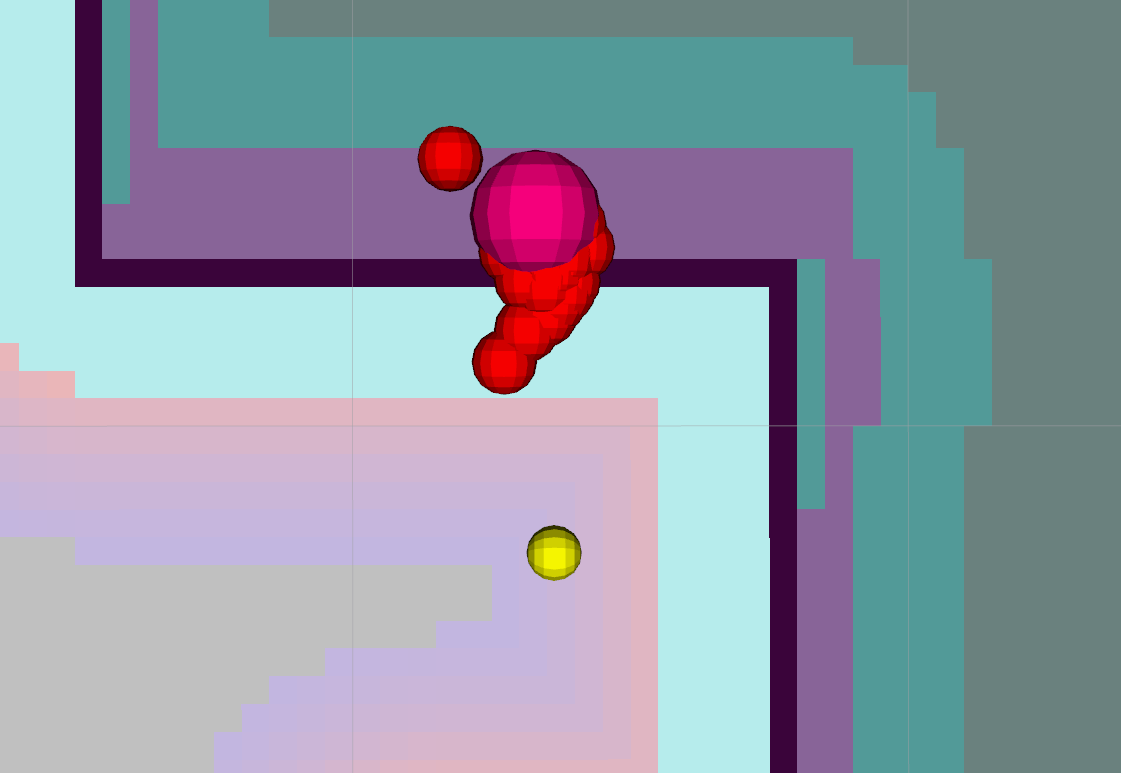
\includegraphics[height=4cm]{images/detections}
		\caption{Inaccurate detection of the object's position due to lack of time synchronization among depth and colour image}
		\label{fig:non_synchronized_raw_detection}
	\end{figure}

	Using camera calibration matrix, focal length and image format can be obtained. Focal length is the distance from the centre of camera coordinate system to image plane. The image format gives us information about width and height of the camera sensor. The camera also has additional information about its position in the world (namely, its position and rotation). \\

	\begin{figure}[h]
		\centering
		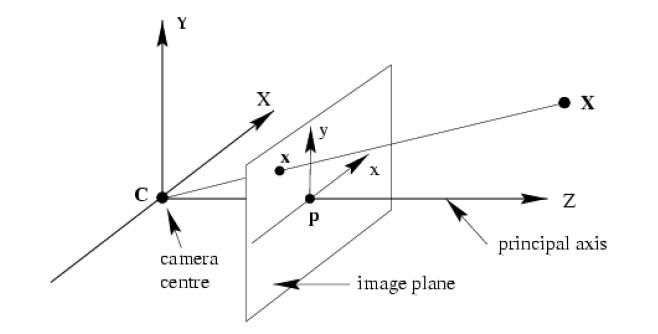
\includegraphics[height=5cm]{images/pinhole_camera_model.png}
		\caption{Pinhole camera model}
		\label{fig:pinhole_camera_model}
	\end{figure}
	
	Assuming that the camera is using pinhole camera model (and the camera calibration matrix is known), a ray can be cast from the centre of the camera coordinate system $C$ to the pixel on image plane, where the object was detected, marked with $x$. This can be seen in the figure \ref{fig:pinhole_camera_model}. Using the computed ray and the distance to the object (namely, vector from camera centre $C$ and the object position $X$), we can compute object's position in a three-dimensional space in camera's coordinate system. \\
	
	After that, we can use a transformation matrix to finally convert the position of the detected object from the camera's coordinate system to the world coordinate system. \\ 
	
	The algorithm explained in this section is used when localizing detected faces and rings. Cylinders are localized using \texttt{PointCloud} information (which is in fact computed from the depth image with a similar approach). \\
	
	\subsection{Faces}
	In this section, we present algorithms that our robot uses to detect faces, compute their orientation in space and classify them.
	
	\subsubsection{Face detection} \label{face_detection_algorithm}
	
	Face detection was done using \texttt{Haar cascade} face detection algorithm. We chose this algorithm because it can be run in real-time and it has a high detection rate. \\
	
	\begin{figure}[h]
		\centering
		
\begin{tikzpicture}
			\fill[lightgray] (0,0.5) rectangle (4,4.5);
			\fill[black] (1,2.75) rectangle (3,3.5);
			\fill[white] (1,2) rectangle (3,2.75);
		\end{tikzpicture}
		\caption{An example of a good Haar feature}
		\label{fig:haar_features}
	\end{figure}
	
	The face images are first cropped to the same size and aligned so that the eyes approximately match. Then, a set of Haar features is generated. Each feature is defined at certain position in the face rectangle and consists of black and white regions (see figure \ref{fig:haar_features}). The value of the feature is computed as as difference between the sum of pixel intensities in the dark regions and the sum of pixel intensities in the light regions. \\
	
	An example Haar feature is displayed in figure \ref{fig:haar_features}. The grey region represents the face region (which fits well in a square). The black and white region is a Haar feature. This specific feature performs well in human eye region detection. It detects the transition from eyes to forehead. \\
	
	Then, for each feature, a simple and fast binary classifier is trained on the training data that can recognize if it is looking at a face or not. Not all features prove to be very good at this task, so the features are ranked by their classification accuracy. With a boosting machine learning algorithm, many weak classifiers (as described above) are used to improve face detection accuracy. A cascade of weak detectors is created such that we start with the most accurate classifier and continue with less accurate ones. This gives the Haar cascade algorithm its real-time ability. For some regions, the first few classifiers detect that there is definitely not a face and the detection can stop. This way, the most processing power is given to the areas that most likely contain a face. \\
	
	The detection is then done with a sliding window method. This simply means that we are evaluating every possible rectangle area in the image. If we want to detect faces of different scales, the image must be resized and the entire algorithm is repeated. So the cascade is crucial for speed here. \\
	
	\subsubsection{Face approaching point computation} \label{face_approaching_points}
	After the face has been detected in an image, its position in the world coordinate system is computed. The approaching point is then calculated using static map information. \textbf{Approaching point} is a point close to the face and directly in front it that the robot must visit to approach the face. \\
	
	To compute the approaching point, the orientation of the detected face must first be determined. In order to do that, we need the static map information. \textbf{Face orientation} is the direction to which the face is looking. \\
	
	\textbf{Static map} is the map of the robot environment. It is used for robot's localization and path computation. In our case it was generated before the task, though algorithms that can explore unknown space exist and could be used to enable our robot to perform this task in unseen environment. In ROS, the map is simply an image with some additional metadata. Each pixel on map represents a small part of the world (in our case, each map pixel represents 5 centimetres in the world).\\
	
	To compute face orientation, its position in the world coordinates is first converted to map coordinates. Then, the corresponding pixel in map is calculated. \\
	
	\begin{figure}[h]
		\centering
		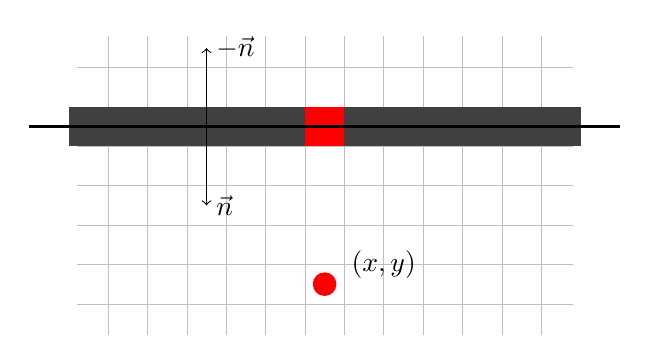
\begin{tikzpicture}
			\draw[step=0.5cm,lightgray,very thin] (0.1,1.1) grid (6.4,4.9);
			\fill[darkgray] (0,3.5) rectangle (6.5,4);
			\fill[red] (3,3.5) rectangle (3.5,4);
			\fill[red] (3.25,1.75) circle (0.15);
			\node[] at (4,2) {$(x, y)$};
			\draw [->] (1.75,3.75) to (1.75,2.75) node [right] {$\vec{n}$};
			\draw [->] (1.75,3.75) to (1.75,4.75) node [right] {$-\vec{n}$};
			\draw[very thick, black] (-0.5,3.75) -- (7,3.75);
		\end{tikzpicture}
		\caption{Face orientation computation}
		\label{fig:orientation_computation}
	\end{figure}
	
	Because of the inaccuracy of the depth sensor, the computed map pixel coordinates don't always lie on the wall. In figure \ref{fig:orientation_computation}, the computed face pixel (pixel, which corresponds to the position of the detected face) is marked with a red circle. \\ 
	
	Using a simple breadth first search in the proximity of the face pixel, the closest pixel from the set of wall pixels (pixels, which correspond to the positions occupied by the walls), is determined. In figure \ref{fig:orientation_computation}, this pixel is coloured red. \\
	
	After the wall pixel has been found, the \texttt{Hough Transform} line finding algorithm is executed on an area around it. The detected line in figure \ref{fig:orientation_computation} is represented in black. If the algorithm finds more than one line, the line which is closest to the wall pixel is selected. The \texttt{Hough Transform} for finding lines will be explained in the section \ref{ring_detection}\\
	
	Because the face is positioned on the wall, one of the wall normals can be chosen as the face orientation. But there are two possible options (as represented in figure \ref{fig:orientation_computation} with labels $\vec{n}$ and $-\vec{n}$), pointing in the opposite directions. The normal that is pointing in the direction of the robot is chosen because otherwise the robot would not be able see the face. \\ 
		
	\subsubsection{Face classification}
	After faces are detected and localized in the world, they have to be identified. For this task we used a pretrained convolutional neural network to create embeddings and then we trained our own model to recognize faces. \\

	The first step in this method is obtaining encodings of our faces by mapping them into an embedding. An embedding is a low-dimensional space to which we map high-dimensional vectors, in this case images. An image gets translated into the embedding by a trained neural network, creating a 128 dimensional vector representation. This is an encoding of the image. In this way we capture some of the semantics of the faces, as similar faces get placed closer together than different faces. \\

	The neural network that we used for our task is a convolutional neural network. It differentiates itself from an ordinary neural network by having convolutional deep layers, which can apply filters to the images, that detect patterns, such as edges and corners and in later layers maybe even specific objects such as eyes or ears. Training of this network is done using triplets. In a single step of the training process, we feed the neural network three images, and thus generate three 128 dimensional encodings. Two images represent faces of the same person, while the third image is a random face, that represents a different person as the one in other two images. Then we tweak the weights in such a way, that encodings of the two faces of the same person get mapped closer together, whereas the third face gets placed farther away. \\

	We could use only one encoding of a certain face, compare it to new faces and still get very good classification results, as was shown in our report for homework 3 with the k-nearest neighbours model for k is 1. However we wanted to make our face recognition more accurate and robust. That is why we trained a separate support vector machine model on the encodings we obtained from the neural network. \\
	
	\subsection{Colour classification} \label{colour_classification}
	The robot must be able to detect the colour of the rings and cylinders. There are six possible classes: black, white, red, green, blue and yellow. \\
	
	In homework 2, we tested different colour spaces and classification models and concluded that the k-nearest neighbours algorithm worked best. The colour space with the highest accuracy in homework was \texttt{HSV} colour model, but in the \texttt{Gazebo simulator}, \texttt{RGB} space worked better. \\
	
	So the colour classifier in the final task uses the \texttt{k-nearest neighbours} algorithm and takes in an input vector in $(red, green, blue)$ format and returns a colour label with one of the six possible classes listed above. \\
	
	Because of the uneven lighting in the \texttt{Gazebo simulator} (and in the real world too), the classifier sometimes returns an incorrect label. We solved this problem by using the robustification process as described in the section \ref{robustification}. Colour classifier is run multiple times on different detections of the same object and the most frequent colour is chosen as the colour of the object. \\
	
	\subsection{Rings}
	In this section, the algorithm for ring detection and its approaching point computation is presented.
	
	\subsubsection{Ring detection} \label{ring_detection}
	When robot finds a woman that is willing to marry Gargamel, it must help him find a ring that she will like. Luckily, she is kind enough to tell us her favourite colour. The robot must then find the ring in that colour, give it to her and ask her to marry Gargamel. \\
	
	But before the ring can be picked up, it must first be detected by the robot. The ring detection is performed on the depth image and the ring colour detection is performed on the rgb image. Again, both images must be synchronized, so the ring can be accurately localized. \\
	
	% I am not sure that the information below is correct
	Depth image is computed from disparity image, which is calculated from the \texttt{Kinect} stereo camera system. The further away the object is, the smaller its disparity will be. Using calibration matrix, depth of each pixel can be approximated from disparity image. Objects that appear further away from the camera have a smaller disparity, which reduces the accuracy of depth computation. To combat this, our algorithm first removes all objects that are more than a certain $threshold$ distance away from the camera. \\
	
	After inaccurate depths are removed, a blob detection algorithm is applied to our depth image. The algorithm finds regions in our image that differ in colour. It actually searches for dark areas (areas that are further away from the camera) in the depth image. Because the inside of the ring is darker than the ring itself, the inner part is considered a blob. But not all blobs are considered rings. We can then apply some domain knowledge to the problem. We know that all the rings are positioned 11 cm above the cubes, so we can filter all blobs that lie below that height. If we look at the ring from any angle, they look elliptical, so the blobs are filtered by their roundness too. \\
	
	\begin{figure}[h]
		\begin{subfigure}{.5\textwidth}
			\centering
			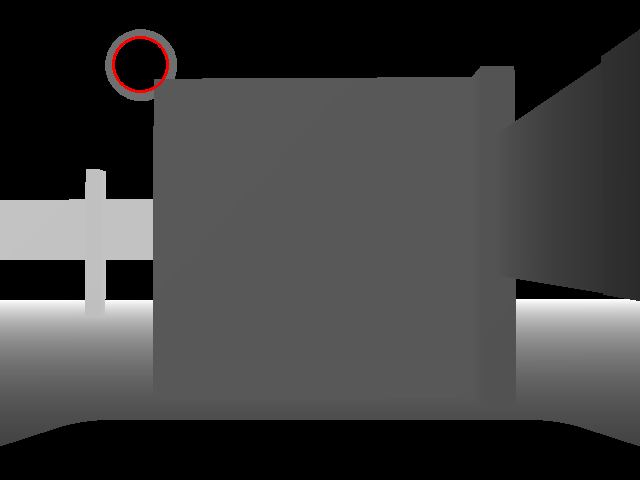
\includegraphics[width=.8\linewidth]{images/ring_detection}
			\caption{Ring detection}
			\label{fig:detected_ring}
		\end{subfigure}
		\begin{subfigure}{.5\textwidth}
			\centering
			
\includegraphics[width=.8\linewidth]{images/ring_detection_cropped}
			\caption{Cropped ring detection}
			\label{fig:detected_ring_cropped}
		\end{subfigure}
		\caption{Ring detection using blob detector}
		\label{fig:ring_detection}
	\end{figure}

	In figure \ref{fig:detected_ring}, we can see an example of a detected ring. Even though the corner of the cube is overlapping with the circle, the ring is still detected. This also presents another problem. To localize the ring, we must know the distance to the ring, but which distance should we use? \\

	Often robot's view of the ring is obstructed by the wall or by a block and sometimes even in such extent that if we created the histogram of the distances on this image, the predominant distance would not be the one to the ring but the one to the wall or a block. To prevent this from happening, we again used some domain knowledge, that the walls and the blocks are white, and we removed from the depth image the parts of detection that correspond to white areas in the rgb image. Now everything is ready to compute the distance to the ring. \\
	
	To compute the distance from camera to the ring, a histogram of distances is created. In figure \ref{fig:distance_histogram}, we can see an example histogram for the figure \ref{fig:detected_ring_cropped} with 24 bins. As we can see, there are two bars that stand out. One of them is the edge of the cube and the other is the ring. A mask is constructed so that only distances that lie in the highest bucket are retained, everything else is removed. \\
	
	\begin{figure}[H]
		\centering
		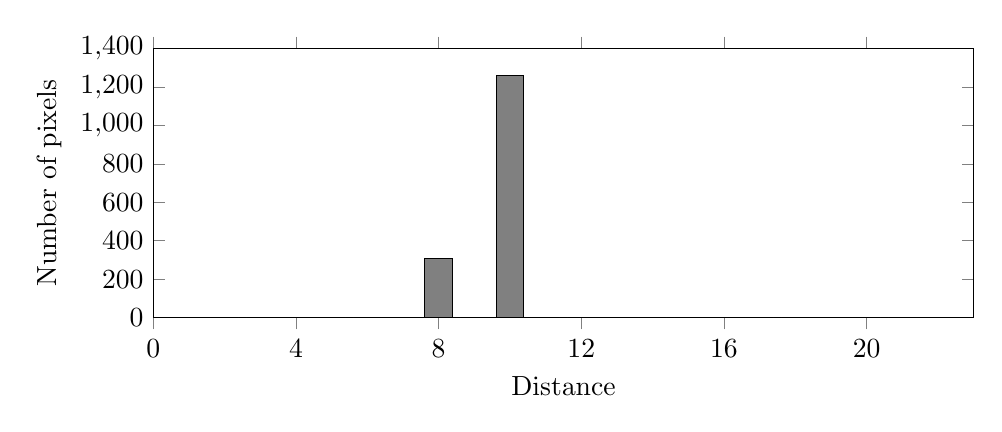
\begin{tikzpicture}
			\begin{axis}[
			ybar,
			xlabel={Distance}, ylabel={Number of pixels},
			xmin=0, xmax=23, ymin=0, ymax=1400,
			xtick={0,4,8,12,16,20,24},
			ytick={0,200,400,600,800,1000,1200,1400,1600},
			width=12cm, height=5cm
			]
			\addplot[fill=gray]
			coordinates {
				(0, 0) (1, 0) (2, 0) (3, 0) (4, 0) (5, 0) (6, 0) (7, 0) (8, 306) (9, 0) (10, 1261) (11, 0) (12, 0) (13, 0) (14, 0) (15, 0) (16, 0) (17, 0) (18, 0) (19, 0) (20, 0) (21, 0) (22, 0) (23, 0) 
			};
			\end{axis}
		\end{tikzpicture}
		\caption{Distance histogram}
		\label{fig:distance_histogram}
	\end{figure}

	The mask is then applied to both, the distance image and the colour image. In figure \ref{fig:masked_colour_ring}, we can see the result of filtering of the \texttt{rgb} colour image using the mask obtained in the previous step. \\

	The distance to the ring is computed as the average of the distances to each pixel in the masked distance image. The algorithm to compute the ring position in world coordinate system is explained in section \ref{pixel_to_world}. \\

	\subsubsection{Ring approaching point computation}
	Computation of approaching points for rings takes advantage of the static map, which provides information about the location of the walls, the unknown space (outside of the map and closed areas inside the map, such as boxes) and the free space, the space through which the robot can move. Using this information and the location of the ring detection we can find the closest wall and move approaching point away from it, in the direction of the normal to the wall. \\

	First we have to find the wall closest to our detection. We can do this by searching for the closest straight line (edge) using \texttt{Hough Transform} algorithm. \texttt{Hough Transform} takes an edge image as the input. \textbf{Edge image} is usually a binary image where one of the binary values 0 and 1 marks the pixels that contain the edge and the other value marks everything else. This kind of image can be obtained by various edge detectors that detect edges by looking for drastic changes in intensity in the original image. \\
	
	Each line from the edge image can then be represented with an equation of the form $y = ax + b$ and mapped to a point $(a, b)$ in \texttt{Hough Space}. Because this system cannot represent the vertical lines since $a$ would be equal to $\infty$, the line is rather represented as $\rho = x\cos(\theta) + y\sin(\theta)$ and mapped to a point $(\theta, \rho)$. Each point from the line therefore produces a cosine curve in \texttt{Hough Space}. If two points lay on the same line, their cosine curves in the \texttt{Hough Space} intersect in one $(\theta, \rho)$ point. The \texttt{Hough Transform} algorithm detects lines by searching for the $(\theta, \rho)$ pairs that record more than some $threshold$ number of intersections. \\

	For each detection we search the area around it for the lines and then find the one that is the closest to the detection. This line is represented with two points, both ends of the line. If we subtract one point from another, we get a vector parallel to the wall. By rotating it by 90 degrees we get a normal $n$ that is perpendicular to the wall. We use static map information to determine whether the neighbouring pixel of the line midpoint in the direction of the $n$ lies in the space accessible to the robot or not. If yes, we take $n$ as our direction vector for setting the approaching point. If not, we take $-n$. \\

	Figure \ref{fig:ring_approaching_point_computation} shows the free space (white) and the inaccessible space (light grey) separated by the wall and the two normals to the wall. Depending on whether the location of the ring is detected correctly (black dot) or incorrectly (red dot) our normal may be either one of the two shown in the Figure \ref{fig:ring_approaching_point_computation}. For setting the approaching point we want a normal to point towards the free space as does $n$ in the figure below. \\

	\definecolor{verylightgray}{gray}{0.90}
	\begin{figure}[H]
		\centering
		\begin{tikzpicture}
			%non-free space
			\fill[verylightgray] (0,4) rectangle (5.5,5.4);

			% grid
			\draw[step=0.5cm,lightgray,very thin] (0.1,2.1) grid (5.4,5.4);

			%wall
			\fill[darkgray] (0,3.5) rectangle (5.5,4);

			% correct ring detection
			\fill[black] (3.25,2.75) circle (0.15);
			%\node[] at (3.5,2.5) {$(x, y)$};

			% incorrect ring detection
			\fill[red] (3.25,4.75) circle (0.15);

			\draw [->] (1.75,3.75) to (1.75,2.75) node [right] {$\vec{n}$};
			\draw [->] (1.75,3.75) to (1.75,4.75) node [right] {$-\vec{n}$};
			\draw[very thick, black] (-0.5,3.75) -- (6,3.75);
		\end{tikzpicture}
		\caption{Computing approaching point for ring}
		\label{fig:ring_approaching_point_computation}
	\end{figure}

	Now we move along the calculated direction vector for 0.45 meters and set this position as the position of the approaching point. Orientation for the approaching point should point towards the line so we just invert the direction vector by multiplying it by $-1$ and set this as the orientation of our approaching point. \\

	\subsubsection{Ring colour detection}
	The ring colour is computed using the mask that we have calculated in section \ref{ring_detection}. The colour  image is filtered so that only ring is left and then the colour is averaged. The average colour is then classified using the algorithm explained in section \ref{colour_classification}. \\
	
	\begin{figure}[h]
		\centering
		
\includegraphics[height=5cm]{images/ring_detection_colour}
		\caption{Masked colour ring}
		\label{fig:masked_colour_ring}
	\end{figure}
		
	\subsection{Cylinder detection} \label{cylinder_detection}
	In this section the algorithm for cylinder detection from point clouds using \texttt{RANSAC} is presented. In short, we first had to remove all larger planes from the point cloud and fit the remaining points to a cylinder model. But first we had to do some preprocessing on the input point cloud data before our algorithm could be run. Namely, making the point cloud sparser in order to reduce the execution time of the algorithm, and then filtering out points beyond some distance from the robot in order to avoid errors in model fitting, caused by the point cloud being too sparse. The points that are far away from the robot are already not very reliable, and by reducing the number of points representing each section we further reduce their accuracy and reliability. \\

	The backbone of our cylinder detection algorithm is fitting a point cloud to a certain model using \texttt{RANdom SAmple Consesus} (\texttt{RANSAC}). This is an iterative method that is used to estimate parameters of a mathematical model from a set of data containing outliers. In every iteration, \texttt{RANSAC} selects a random subsample of the input data. These points are then considered inliers and the hypothesis is tested in a few steps. First the model is fitted to the inliers, then all data points are tested against the fitted model, and if they fit well, they are also considered inliers. After that the model is re-estimated from the original and new inliers and finally, it is evaluated by estimating the error of the inliers relative to the model. After a fixed number of iterations, the best model is chosen. \\
	
	\subsubsection{Removal of planes}
	To be able to detect cylinders efficiently and robustly, we first need to remove all planes from the point cloud in order to reduce the computational load and avoid many flat surfaces and corners from being detected as cylinders. We do this by iteratively fitting the point cloud to a plane model with \texttt{RANSAC}, as explained above, and then removing all the inliers from the point cloud. This way we remove all large planes in the point cloud that have more inliers than some empirically set threshold. \\
	
	A threshold is used so that the points that are part of the cylinders are retained, because a small enough area of the cylinder might be considered a plane, and thus be removed from the point cloud. This parameter had to be fine tuned in order to remove as many planes from the point cloud, but also keep the cylinder inliers. \\

	\subsubsection{Cylinder detection}
	After all or most of the planes have been removed from the point cloud, we can detect cylinders. The method for this is very similar to the one used for detecting planes, but instead of fitting a point cloud to a plane, we fit it to a cylinder. This is trickier, because cylinders are more complex objects with more parameters and thus, it is harder to fit the points to the model. The parameters for this method had to be carefully chosen in order to accurately detect cylinders and avoid incorrect detections such as corners. \\

	We chose to only detect one cylinder in a point cloud. Firstly, because usually they are relatively far apart, so there is no fear that we could miss one, and secondly, because the farther the object is from the robot, the sparser is the point cloud and consequently more errors are present, such as mistaking a cylinder for a plane or vice versa. \\
	
	\subsubsection{Cylinder approaching point computation}
	The cylinder approaching point computation is not as difficult as the one for the faces. If a cylinder has been detected from the current robot's position, that means that the robot must have had a clear view of the cylinder. Because of that, the approaching point can be computed as a point on the line connecting the robot and the cylinder. \\
	
	A point that lies 0.6 metres from the centroid of the cylinder on this line is selected as the approaching point. If the point can't be reached (that is, if it is too close to the wall), approaching point is repositioned so that there is enough space for the robot to visit the point. This is done by finding the closest wall on the map and then moving the point in the opposite direction. This is repeated until there is no wall too close to the point. \\
	
	\subsection{Robustification} \label{robustification}
	The sensors are not 100\% accurate, so we have to take into account some possible errors. For example, when an object is detected, the depth sensor might compute the distance inaccurately, or the robot may not have been localized. Sometimes, detectors might return false positives and so on. \\
	
	To combat this problem, a robustification is performed on the detected objects. The object detectors send detections to their respective robustifiers, which collect data and determine whether the detection is a true positive or not. \\
	
	For detection to be considered a true positive, the following must hold true:
	\begin{enumerate}
		\item Detected object was detected at least \texttt{threshold} times.
		\item There is at least a \texttt{minimum distance} meters distance between this detection and every other previous true positive.
	\end{enumerate}

	If two detections are close enough (the distance between them is less than \texttt{minimum distance}), they are considered the same object. The positions of those two detections in the world are then averaged, so the calculated object position is closer to its actual position in space. The object colour is also chosen as the most frequent detected colour. \\
	
	\begin{figure}[h]
		\centering
		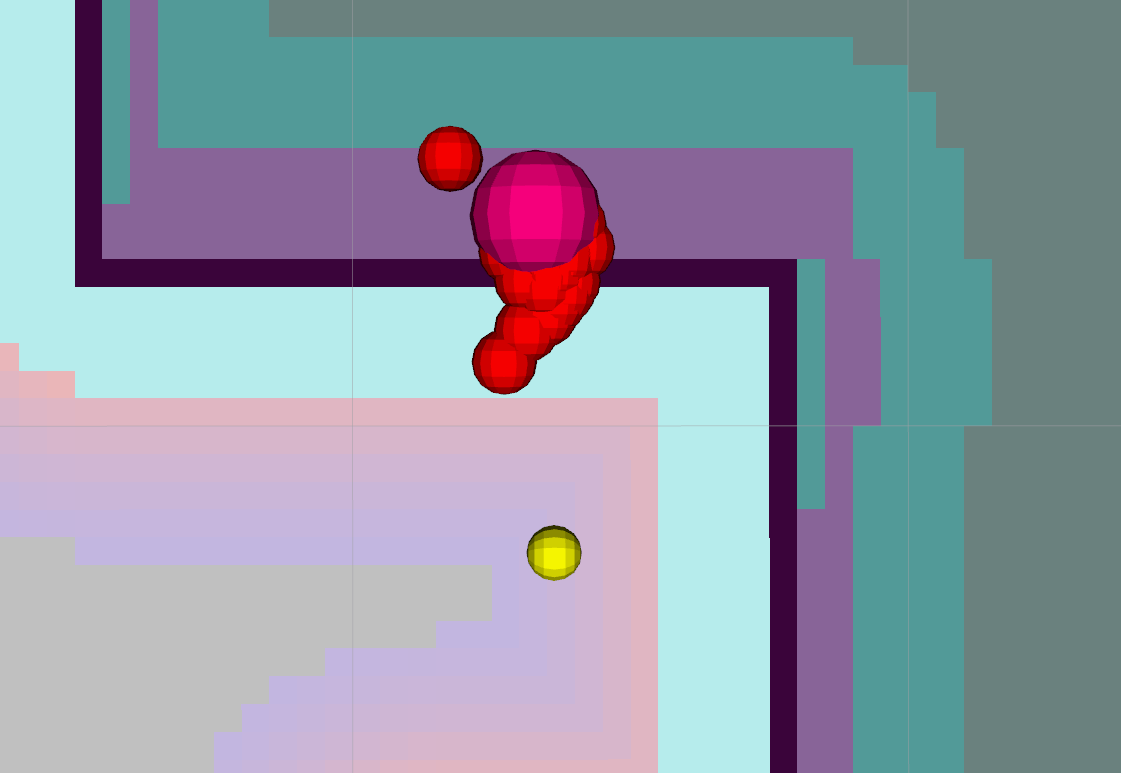
\includegraphics[height=4cm]{images/detections}
		\caption{Many inaccurate object detections}
		\label{fig:inaccurate_detections}
	\end{figure}

	Figure \ref{fig:inaccurate_detections} shows why the robustification process is needed. Face detector works very fast, but the localization isn't that accurate. Each red sphere represents one face detection. By averaging many face detections, the pink sphere position is obtained. As we can see, the the averaged position is much closer to the real face position (which is in this case on the wall near this averaged position) than each individual detection. The distance between the farthest points in figure \ref{fig:inaccurate_detections} is 0.3 metres, which is another reason why we think robustification process is needed. \\
	
	It should also be noted that similar process is applied to the approaching points. Approaching point is computed for each face detection and as positions of the face detections are averaged, approaching points are averaged as well. In figure \ref{fig:inaccurate_detections}, this point is yellow. \\
		
	\subsection{Smart exploration of space} \label{smart_exploration}
	There are two ways to determine some goals for space exploration. Either you hard-code a list of goals or you create a system that automatically sets the goals based on the shape of the map. Hard-coding is almost never a good idea, se we went with the latter. \\

	Our algorithm uses static map as the input. First, the contrast between the walls or unknown space, and the space where robot can move, is amplified. After that a morphological operation of closing is performed to smooth out the corners which robot can't reach because of its circular shape. \\
	
	The part containing the relevant map is cropped out of the whole image as the other empty parts are not needed for rest of the process. We then find the corners with \texttt{Harris corner detector} and then apply the \texttt{non maxima suppression} to only keep the actual corners. The corners are corners in the walls and obstacles and also the ends of the walls. \\
	
	An edge is a sudden change in brightness and a corner is the point where two edges meet. Corners are the points, where gradient change is big in all directions. Harris corner detector works on a grey-scale image, smoothed by a \texttt{Gaussian filter} (removes any noise). For each pixel in the image, it considers a 3x3 window around it and uses derivatives to computes a \texttt{Harris value} for it. \texttt{Harris value} is a score which tells how likely does the pixel contain a corner. \texttt{Non maxima suppression} is used to only declare corners in the pixels, whose score is the local maximum of the certain window and also exceed some threshold value. \\

	With the list of corners in the map ready, we can perform \texttt{Delaunay triangulation} to split the space without obstacles into triangles. \texttt{Delaunay triangulation} is a special kind of triangulation, where no point from the set on which the triangulation is performed is inside the circumcircle of any triangle in the triangulation. Another property of the \texttt{Delaunay triangulation} is that it maximizes the minimum angle in the triangles and thus create more even distribution of the area. \\

	For each triangle, our algorithm find its centroid - the centre of the circumcircle. If we were to connect the centroids, we would obtain a so called \texttt{Voronoi diagram}, a special partition of the plane into regions. Each region contains all of the points that are closer to the seed inside this region, in our case a corner, than to any other seed (corner). The points from the \texttt{Delaunay triangulation} (centroids) are therefore as far away from all walls as possible. This makes them great points for space exploration as they are far from the obstacles and somewhat evenly distributed across the map. \\

	We have to be careful as centroids from the \texttt{Delaunay triangulation} will also be set in narrow passageways to which robot may not have access. And sometimes, two points might end up very close together, which isn't ideal for the exploration. \\
	
	To eliminate the second problem, we use \texttt{hierarchical clustering} with the minimum distance as the stopping criteria. This merges any points that are too close together into one, their average. It does so hierarchically, in each iteration it merges only the two points that are the closest. \\
	
	This step can sometimes also solve the first problem. To be sure that the robot can reach all of the exploration goals, we check if any goal is too close to any wall and if so, move it into the opposite direction, away from the wall, if possible. \\

	In the figure below, we can see the \texttt{Delaunay triangulation} of our map in green and the centroids in red. The points in blue represent the exploration goals after \texttt{hierarchical clustering} and moving points away from the walls. \\

	\begin{figure}[h]
		\begin{subfigure}{.5\textwidth}
			\centering
			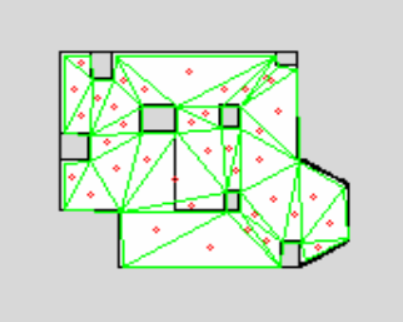
\includegraphics[height=5cm]{images/before}
			\caption{Before processing}
			\label{fig:before_clustering}
		\end{subfigure}
		\begin{subfigure}{.5\textwidth}
			\centering
			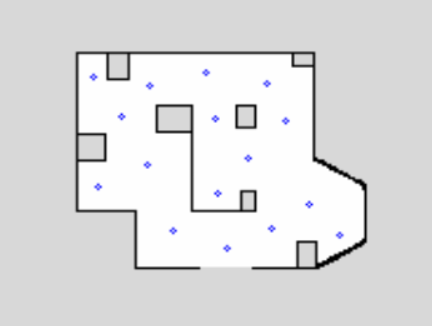
\includegraphics[height=5cm]{images/after}
			\caption{After processing}
			\label{fig:after_clustering}
		\end{subfigure}
		\caption{\texttt{Delaunay triangulation} and exploration goals before (a) and after the \texttt{hierarchical clustering} and moving unreachable goals to reachable position (b).}
		\label{fig:exploration_goals}
	\end{figure}
	
	\subsection{Fine movement} \label{fine_movement}
	Fine movement is a special way in which our robot can move. It is used when the default movement wouldn't be able to get us to the goal even though the goal is reachable.  \\

	The \texttt{move\_base} package can be used with \texttt{ROS} to move the mobile base around the map. It uses local and global planner information to avoid obstacles and try to reach the given goal. If it fails to reach the goal, it tries to clear its local map. If that fails, the robot stops trying to reach the goal and notifies us that it has failed to move to the goal. \\
	
	The most common reason for failure is that the goal is too close to any wall in our world. The robot builds a costmap of its environment, where the closer the position is to the wall, the highest cost it has. This way a robot can avoid obstacles and plan the path from point A to point B. The robot builds a costmap in a way that it makes sure not to bump into anything, which means it also takes into account all possible errors in data from its detectors. This means that some of the points that the robot can reach in reality unfortunately fall into the high-cost area and so the default movement cannot get us there because the risk of bumping into something is too high. \\

	In our final task, the robot had to be able to pick up rings that are positioned very close to the wall and get very close to the cylinders so that it could reach above it and toss a coin. Both required positions are so close to the obstacle/wall, that the default movement component is unable to reach the goal. To do that, odometry data must be used and combined with \texttt{Twist} messages to move the robot \say{manually}. \\

	Fine movement that we implemented works as follows. In the first step we obtain the current position of the robot and calculate its distance to the goal. Then we calculate the difference between the robot's orientation and the direction that would point from the robot's position to the position of the goal; let's call it \textbf{direction to goal}. Then we check whether the robot is already near enough to the position of the goal. There is a certain threshold set and if the distance between the robot and the goal is below this threshold, we consider the robot to have reached the position of the goal. This helps in case a goal is too close to the wall for the centre of the robot to reach it without crashing into any obstacles. \\
	
	If we are not close enough, we send a \texttt{Twist} message to move the robot in the direction to goal and then repeat the first step. \\
	
	If we are close enough, we check the difference between the robot's current orientation and the orientation of the goal. If it is below a certain $threshold$ for orientation, we assume the orientation is correct and the robot has successfully reached the goal, so we can move on to perform other tasks. If the orientation is not as desired, we send a \texttt{Twist} message with the linear components equal to 0 so that the robot does not move forward but only spins around on the spot, and the angular components set such that it reduces the difference in robot's orientation and that of a goal. \\

	This behaviour is shown in the figure \ref{fig:fine_movement_figure} below. Step 1 shows the robot and the goal at the start. In the step 2 we can see that the robot has turned towards the goal and will proceed forward in this direction. Step 3 shows the robot in the moment it reaches the position of the goal and in step 4 we can see the robot turning to match the orientation of the goal. In step 4, the goal is successfully reached. \\
	
	\begin{figure}[H]
		\begin{subfigure}{.5\textwidth}
			\centering
			\begin{tikzpicture}
			\draw[lightgray, very thin] (-0.5, -0.5) rectangle (4.5, 4.5);
			% Robot
			\draw[thick] (1.5, 1) circle (0.4);
			\draw [->, thick] (1.85951761852, 1.17534845872) to (2.3987940463, 1.43837114679) node [right] {};
			\fill[black] (1.5, 1) circle (0.025);
			% Ring
			\fill[black] (2, 3) circle (0.1);
			\draw [->] (2, 3) to (2 - 0.3, 3) node [right] {};
			\end{tikzpicture}
			\caption{Step 1}
		\end{subfigure}
		\begin{subfigure}{.5\textwidth}
			\centering
			\begin{tikzpicture}
			\draw[lightgray, very thin] (-0.5, -0.5) rectangle (4.5, 4.5);
			% Robot
			\draw[thick] (1.5, 1) circle (0.4);
			\draw [->, thick] (1.59701425001, 1.38805700006) to (1.74253562504, 1.97014250015) node [right] {};
			\fill[black] (1.5, 1) circle (0.025);
			% Ring
			\fill[black] (2, 3) circle (0.1);
			\draw [->] (2, 3) to (2 - 0.3, 3) node [right] {};
			\end{tikzpicture}
			\caption{Step 2}
		\end{subfigure}
		\begin{subfigure}{.5\textwidth}
			\centering
			\begin{tikzpicture}
			\draw[lightgray, very thin] (-0.5, -0.5) rectangle (4.5, 4.5);
			% Robot
			\draw[thick] (2, 3) circle (0.4);
			\draw [->, thick] (0.5 + 1.59701425001, 2 + 1.38805700006) to (0.5 + 1.74253562504, 2 + 1.97014250015) node [right] {};
			% Ring
			\fill[black] (2, 3) circle (0.1);
			\draw [->] (2, 3) to (2 - 0.3, 3) node [right] {};
			\end{tikzpicture}
			\caption{Step 3}
		\end{subfigure}
		\begin{subfigure}{.5\textwidth}
			\centering
			\begin{tikzpicture}
			\draw[lightgray, very thin] (-0.5, -0.5) rectangle (4.5, 4.5);
			% Robot
			\draw[thick] (2, 3) circle (0.4);
			\draw [->, thick] (2 - 0.4, 3) to (0.5 + 2 - 1 - 0.4, 3) node [right] {};
			% Ring
			\fill[black] (2, 3) circle (0.1);
			\draw [->] (2, 3) to (2 - 0.3, 3) node [right] {};
			\end{tikzpicture}
			\caption{Step 4}
		\end{subfigure}
		\caption{Fine movement}
		\label{fig:fine_movement_figure}
	\end{figure}

	At first we implemented fine movement that included more advanced path planning with the \texttt{A*} algorithm. We realized that it would be very slow to travel far with fine movement so we set up approaching points for the objects that needed approaching with fine movement (cylinders and rings). These points enabled our robot to quickly get close to the goal with the standard version of the movement and then switch to the fine movement to precisely and carefully approach the object of interest. Having these approaching points, there was no need for such complex path planning so we replaced the initial algorithm with the simpler one, as described above. \\
	
	Note that this implementation assumes that there is a clear view of the goal from the point at which the fine movement begins - there should be no obstacles on the line connecting the starting point and the goal and in the area of the robot's radius to the both sides of this line. \\

	Even though fine movement allows us to reach the points close to the wall or obstacles, it does not, however, allow us to reach the points that are closer to a wall or an obstacle than the size of the robot's radius. For this reason, we defined two additional types of approaching points specifically for the fine movement. Both Toss-a-coin approaching point and Pick-up-the-ring approaching point are computed in the \texttt{Brain} component. \\

	\subsubsection{Toss-a-coin approaching point} \label{toss-a-coin-point}
	Toss-a-coin approaching point is a point near the cylinder and orientated towards the cylinder from which we can reach above the cylinder with the robotic arm and simulate tossing a coin into the wishing well. The point is set halfway from the cylinder approaching point to the detected centre of the cylinder. Orientation for this point is set equal to that of the cylinder approaching point. \\

	\subsubsection{Pick-up-the-ring approaching point} \label{pick-up-the-ring-point}
	Pick-up-the-ring approaching point is a point near the ring from which the ring can be picked up by the robotic arm that is mounted on top of the robot. This point is located halfway between the ring approaching point and the detected ring location. Orientation of this point is set to such that the robot is below the ring, having its right side next to the wall to which the ring is \say{attached}. This means the orientation of the ring approaching point should be rotated 90 degrees counter clockwise (to the robot's left). \\
	
	\subsection{Robot's behaviour}
	
	\begin{figure}[H]
		\centering
		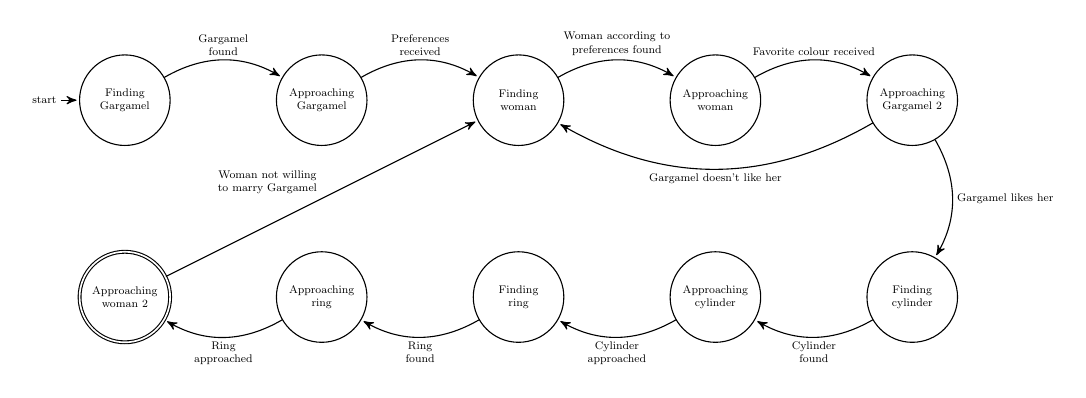
\begin{tikzpicture}[->, >=stealth', shorten >=1pt, auto, node distance=5cm, scale=0.5, 
		transform shape, align=center, state/.style={circle, draw, minimum size=2.3cm}]
		
			\tikzset{every edge/.append style={font=\footnotesize}}
			\tikzset{every node/.append style={font=\footnotesize}}
			
			\node[initial,state] 	(FG) {Finding \\ Gargamel};
	 		\node[state] (AG) 		[right of=FG] {Approaching \\ Gargamel};
  			\node[state]         	(FW) [right of=AG] {Finding \\ woman};
  			\node[state]         	(AW) [right of=FW] {Approaching \\ woman};
  			\node[state]         	(AG2) [right of=AW] {Approaching \\ Gargamel 2};
  			\node[state]         	(FC) [below of=AG2] {Finding \\ cylinder};
  			\node[state]         	(AC) [left of=FC] {Approaching \\ cylinder};
  			\node[state]         	(FR) [left of=AC] {Finding \\ ring};
  			\node[state]         	(AR) [left of=FR] {Approaching \\ ring};
  			\node[accepting, state] (AW2) [left of=AR] {Approaching \\ woman 2};
  			
  			\path (FG) edge[bend left] node {Gargamel \\ found} (AG);
  			
  			\path (AG) edge[bend left] node {Preferences \\ received} (FW);
  			\path (FW) edge[bend left] node {Woman according to \\ preferences found} (AW);
  			\path (AW) edge[bend left] node {Favorite colour received} (AG2);
  			\path (AG2) edge[bend left] node {Gargamel doesn't like her} (FW);
  			
  			\path (AG2) edge[bend left] node {Gargamel likes her} (FC);
  			\path (FC) edge[bend left] node {Cylinder \\ found} (AC);
  			\path (AC) edge[bend left] node {Cylinder \\ approached} (FR);
  			\path (FR) edge[bend left] node {Ring \\ found} (AR);
  			\path (AR) edge[bend left] node {Ring \\ approached} (AW2);
  			
  			\path (AW2) edge[] node {Woman not willing \\ to marry Gargamel} (FW);
  			
		\end{tikzpicture}
		\caption{Finite state automaton}
		\label{fig:finite_state_automaton}
	\end{figure}

	In this part, the robot's behaviour and decision making will be explained. In order to make robot's artificial intelligence implementation easily understandable and straightforward, we decided to use finite state automata. We defined ten states, that can be seen in the figure \ref{fig:finite_state_automaton}, most of them having only one outgoing edge except for the two nodes that have two outgoing edges. \\

	\texttt{Finding Gargamel}: In this initial state of the automaton, the robot travels around the map and memorizes any objects of interest that it detects, until it finds Gargamel. Then the robot transitions into the second state. \\

	\texttt{Approaching Gargamel}: Here we first instruct the robot to approach Gargamel. When the specified approaching point is reached, the robot asks Gargamel about his preferences about women. The robot then listens for the answer. If it fails to understand the answer twice, it prompts us to input it manually through the terminal. Once Gargamel's preferences are received, the robot transitions to the next state. \\

	\texttt{Finding woman}: In this state, the robot has to find a woman that matches Gargamel's preferences. We first check if we have already detected any women with such characteristics and if so, we choose the first one and proceed to the next state, in which we approach the woman. Otherwise we instruct the robot to explore the map until it finds a suitable woman. \\

	\texttt{Approaching woman}: In this state, the robot approaches the woman we found in the previous state. After it reaches the approaching point, it inquires about her favourite colour. The logic of handling speech recognition is the same as in \texttt{Approaching Gargamel} state. \\

	\texttt{Approaching Gargamel 2}: With this newly collected information about the woman's favourite colour, the robot returns to Gargamel. Woman's picture is shown in \texttt{rviz} while the robot waits for Gargamel's response, whether he likes this woman or not. Based on the received information, we have two possible transitions. If Gargamel likes this woman, we proceed to next state, if he doesn't like her, we return to the \texttt{Finding woman} state, where we search for a new woman with characteristics that Gargamel likes. \\

	\texttt{Finding cylinder}: Robot's next task is to find a cylinder in the woman's favourite colour. Here we have two options, if a cylinder of the specified colour has already been detected, we proceed to the next state, otherwise the robot is instructed to explore the map until it finds a suitable cylinder. \\

	\texttt{Approaching cylinder}: After an appropriate cylinder has been found, the robot's next step is to approach it and extend the mechanical arm, which represents tossing a coin into a wishing well. This is achieved in the following manner. The robot first approaches the cylinder, then it has to get closer to the cylinder, using fine movement. When it is close enough and facing the cylinder, it finally extends the arm. After that, the robot returns to the approaching point and continues to the next state. \\

	\texttt{Finding ring}: This next task is very similar to the one in the \texttt{Finding cylinder} state, except that the robot is searching for a ring of a specified colour. When appropriate ring is found, we continue to the next state. \\

	\texttt{Approaching ring}: After a suitable ring has been found, the robot has to approach it and extend its arm towards it, simulating picking up the ring. This is achieved by approaching the ring, getting closer and into the right position using fine movement and extending the arm towards the ring, similarly as in the \texttt{Approaching cylinder} state. Once the robot reaches the ring, it returns to the approaching point and continues to the next state. \\

	\texttt{Approaching woman 2}: This is the accepting state of this automaton. The robot's job is to approach the chosen woman again and ask her if she is willing to marry Gargamel. If her answer is yes, the robot has finished his task. If her answer is no, the robot returns back to the \texttt{Finding woman} state and searches for a new woman with desired characteristics. \\
	
	\section{Implementation and integration}
	In this section, the implementation of the algorithms explained in section \ref{methods} will be discussed. To solve our task, the following architecture, presented in figure \ref{fig:final_architecture}, was designed. We tried to keep the entire project as modular as possible, not only because this is the \texttt{ROS} operating system's philosophy, but also because three different people needed to work on the same project at once. \\
	
	This proved to be very difficult because nodes are so interconnected, that if any part of the system didn't work as intended, it seemed as if nothing worked. Some parts of the system were discussed beforehand, but as the tasks became more difficult, the architecture had to be changed in order to solve them. \\ 
	
	\begin{figure}[h]
		\centering
		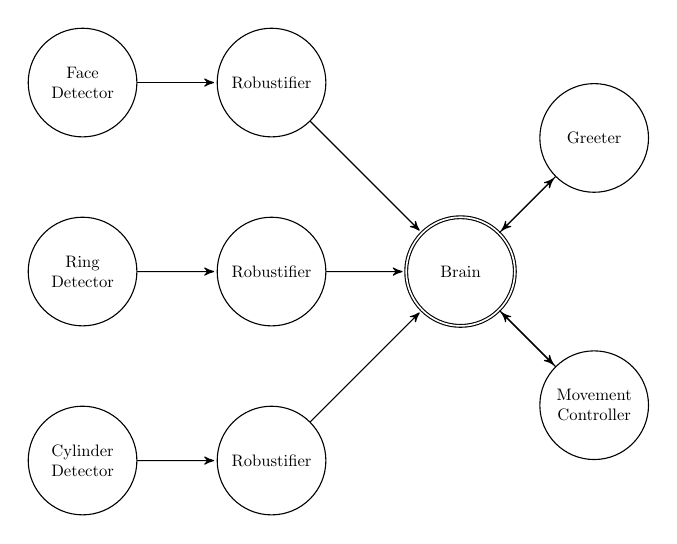
\begin{tikzpicture}[->, >=stealth', shorten >=1pt, auto, node distance=4cm, scale=0.6, transform shape, align=center, state/.style={circle, draw, minimum size=2.3cm}]
			\node[state] 	(FD) {Face \\ Detector};
			\node[state] 	(RD) [below of=FD]{Ring \\ Detector};
			\node[state] 	(CD) [below of=RD]{Cylinder \\ Detector};
			\node[state] 	(FR) [right of=FD] {Robustifier};
			\node[state]	(RR) [right of=RD] {Robustifier};
			\node[state] 	(CR) [right of=CD] {Robustifier};
			\node[state, accepting] 	(BR) [right of=RR] {Brain};
			\node[state] 	(GR) [above right of=BR] {Greeter};
			\node[state] 	(MC) [below right of=BR] {Movement \\ Controller};

			\path (FD) edge (FR);
			\path (RD) edge (RR);
			\path (CD) edge (CR);
			\path (FR) edge (BR);
			\path (RR) edge (BR);
			\path (CR) edge (BR);
			\path (BR) edge (MC);
			\path (MC) edge (BR);
			\path (BR) edge (GR);
			\path (GR) edge (BR);
			
		\end{tikzpicture}
		\caption{Final architecture}
		\label{fig:final_architecture}
	\end{figure}
	
	\subsection{Object detectors}
	There are three different nodes responsible for object detections. Face and ring detectors are using rgb and depth images and the cylinder detector is using point cloud and rgb image to detect objects in our world. \\
	
	All three object detectors are publishing a custom \texttt{ObjectDetection} message type. The \texttt{Robustifier} component subscribes to this type of message and tries to minimize the number of false positives. The robustification process is also the reason why we felt the need for and created the \texttt{ObjectDetection} message type. \\
	
	\subsubsection{ObjectDetection message} \label{objectDetection}
	The object detection message contains the following information.
	\begin{enumerate}
		\item \texttt{Header header}, which contains the time stamp of the detection and other metadata.
		\item \texttt{string id}, which is a unique number used to identify the detection.
		\item \texttt{Image image}, which is an image of the object.
		\item \texttt{Pose object\_pose}, which represents the object position in world coordinate frame.
		\item \texttt{Pose approaching\_point\_pose}, which is a point that the robot has to visit in order to complete the task.
		\item \texttt{string color}, which represent the object's average colour label that the colour classifier computed.
		\item \texttt{string face\_label}, which carries the label of the face that our face classifier recognized.
		\item \texttt{string type}, which represents the type of the detected object (it can be either \texttt{"face"}, \texttt{"ring"} or \texttt{"cylinder"}).
		\item \texttt{string barcode\_data}, which carries the url that the QR code contained. It was introduced when we were using QR codes to get information about faces, but it became unnecessary after the face classifier was implemented.
	\end{enumerate}
	
	\subsubsection{Face detector node}
	The face detector is responsible for detecting and localizing faces. To do that, it first synchronizes received rgb and depth images using the \texttt{Time Synchronizer} class in \texttt{message\_filters} package. \\

	After both, rgb and depth images are received, it uses the \texttt{Haar cascade} algorithm explained in section \ref{face_detection_algorithm} to detect faces. If a face has been found, it tries to compute its world position. This is done using ray casting from the camera centre, through the face centre pixel in the image plane as explained in section \ref{pixel_to_world}. \\

	After the face is localized, Approaching point is computed. Approaching point is a point that is positioned directly in front of the face. Because the faces are positioned on the walls, the closest wall to the face is found. Then, the wall normal is computed as explained in section \ref{face_approaching_points}. The Approaching point is positioned 0.6 metres from the face position in the direction of the face orientation. \\

	\subsubsection{Ring detector node}
	Ring detector is a node that is responsible for ring detection and localization. It works similarly to the face detector node. First, it synchronizes depth and rgb images. Then it uses the ring detection algorithm as explained in section \ref{ring_detection}. Ring localization is done using the algorithm explained in section \ref{pixel_to_world}. \\
	
	Ring orientation is determined using similar algorithm as explained in section \ref{face_approaching_points}, but instead of finding the normal of the wall, its direction is chosen as ring the orientation. \\
	
	\subsubsection{Cylinder detector node}
	Cylinder detector is a node that is responsible for detecting and localizing the cylinders. It first synchronizes depth and rgb images. Then it uses the cylinder detection algorithm that is explained in section \ref{cylinder_detection}. \\

	\subsection{Robustifier}
	For each object detector, a new \texttt{Robustifier} node is created. Each \texttt{Robustifier} node is listening for different object detections. The detections are then grouped together using the algorithm as explained in section \ref{robustification}. When number of detections sent to the \texttt{Robustifier} node exceeds the threshold value, the detection is considered a true positive and is sent to the \texttt{Brain} node. \\
	
	But this is not the end of the robustification process. For each new detection, average positions are calculated again, and updated results are sent to the \texttt{Brain} node as well as and used to update the positions of the markers in \texttt{rviz} as well. \\
	
	\subsection{Brain}
	\texttt{Brain} is a node that is responsible for solving the main part of the task. \\
	
	It is the main node of our project that brings all other functionalities into one complete whole. It subscribes to robustified object detections and saves them. Then it uses these detections and the behavior logic to complete the task. \\
	
	\subsection{Movement controller}
	\texttt{Movement controller} is an object, that allows our robot to interact with its environment. It allows it to move and explore the space and use its robotic arm to grab items. It works using a series of tasks, which the robot executes one by one. When the task is finished, a callback function is used to notify the robot that the action is completed. \\

	\subsubsection{Movement tasks}
	Each task represents one action that the robot can do.

	\begin{enumerate}
		\item \texttt{Localization task} is a task that is run at the beginning. The robot knows its approximate location in the space, but before it can move around the environment, it must pinpoint its exact location. This task rotates the robot around its vertical axis for one full rotation using odometry information. The robot uses depth information to localize itself using adaptive Monte Carlo localization algorithm.
		\item \texttt{Approaching task} is a task that drives the robot around its environment using the standard \texttt{move\_base} package.
		\item \texttt{Fine approaching task} is a task similar to the \texttt{Approaching task} except it uses our fine movement algorithm as explained in section \ref{fine_movement}. This task is always performed to move the robot between the position reached by approaching task and one of the special approaching points, \texttt{Toss-a-coin approaching point} and \texttt{Pick-up-the-ring approaching point}.
		\item \texttt{Wandering task} is a task where the robot is exploring its environment, searching for faces, rings and cylinders. It uses the points generated by the algorithm for smart exploration of space, described in the section \ref{smart_exploration}. This task can be cancelled at any time so the robot can visit detected objects, if needed.
		\item \texttt{Arm task} is a task where the robot uses its pincher arm that is mounted on top of it. This task is used to toss a coin into a wishing well (moving the robot arm above a cylinder) or pick up a ring that is floating above the ground.
	\end{enumerate}

	The \texttt{movement controller} uses an ordered list of tasks. If the \texttt{brain} component chooses, it can cancel the current task, reorder its task and insert new task to be executed either after all tasks have finished or right at this moment. \\
	
	\subsection{Greeter}
	Greeter is a node that uses \texttt{SoundClient} for speech synthesis. It is used whenever we want robot to say something out loud. \\
	
	\section{Results}

	After countless hours, Erazem was finally able to perform the task. We encountered a bunch of problems on the way, the biggest one being the task of approaching the rings. We spent at least a week trying to reliably set the approaching points for the rings, wrote many different algorithms for this task, tried improving ring detection in several ways, changed how the fine movement works multiple times, set up various robustification processes for both detections and approaching points, and even even set up a two layer robustification process. But all that with no definite success. In the presentation of the last task our robot did not set the points correctly for all of the rings and consequently couldn't approach some of them correctly. \\

	In the final presentation some things didn't go as planned:
	\begin{itemize}
		
		\item Erazem took forever to toss a coin into the red cylinder, the second one that we had to approach. What went wrong was the robot wasn't able to reach the desired orientation on a Toss-a-coin approaching point and as we didn't implement a time-out for this task, it got stuck there. Toss-a-coin approaching point is set as the midpoint of the line connecting the centre of the cylinder and its approaching point (see section \ref{toss-a-coin-point}). \\
		Since cylinder detections are not always accurate the robustifier averages them. The problem here was, that robustifier also updates the presumed cylinder position for every detection it receives, and in this case the \say{true positive} for the red cylinder was not accurate. The Toss-a-coin approaching point ended up a bit too close to the cylinder, as the robot was able to reach it's position but was unable to turn into the right direction. \\
		
		\item Because of the error above, Erazem didn't have a chance to fail at picking up the red ring but it certainly would've had as the approaching point for the ring wasn't set correctly. Our first implementation of the fine approaching could handle examples like this one, but it wasn't very practical as it was slow, so we replaced it with a simpler version that uses approaching points and then assumes the way in the direction straight to the Pick-up-the-ring approaching point is free (see sections \ref{fine_movement} and \ref{pick-up-the-ring-point}). \\
		As the approaching point was not set correctly, this path was not free and the robot would have bumped into the wall and messed up his odometry. The reason for the incorrect position of the approaching point are inaccurate detections of the red ring's position (which occur when the robot is moving or rotating fast). Because of this, some approaching points were positioned in the wrong direction and as they were averaged in the robustification process, the calculated position of the approaching point was not in the right place.
		
		\item We also forgot that we had to show the image of the woman to Gargamel before asking him if he liked her or not. This was not an error in the code but just something we forgot to implement. Our architecture was ready to perform this task (see section \ref{objectDetection}) but at the end we forgot to show the image.
		
		\item At one point our robot needed a bit longer to set it's new goal as the goal it was trying to set was not reachable. The reason is, one of the points our smart space exploration algorithm sets was positioned near the green cylinder. This algorithm uses only the shape of the map as the robot cannot know the positions of the cylinders in advance. However, cylinders take up some space and in this case robot's calculated that the point was too close to the obstacle to be reached. \\
		This error was something we have foreseen so we handled such situations as follows. If the path to the goal cannot be found, try again. If you already tried three times, move this goal to the end of the queue and proceed with finding path to the next goal in the queue. This meant our robot stopped for about 5 seconds but then proceeded with the task as if nothing had happened.
	\end{itemize}

	On the presentation of the final task we could see that Erazem was an excellent match maker and was able to perform every part of his job. But since he is still somewhat of a newbie, he made some rookie mistakes and didn't always know how to best handle the situation when things didn't go as planned.

	\section{Division of work}
	Since this project is extensive, we tried to build it from several modules to make it more manageable. Despite this, it was impossible to just divide the work exactly by modules as they are still very interconnected. It is also more convenient and fast to fix some error or slightly change an algorithm by yourself as you notice the need for it, than to explain everything to the person, who initially built the node, and wait for them to make the changes the next time they sit at their computer. For these reasons, the division of the work is not very clean and straightforward. There is a also a lot of work that is invisible as it includes algorithms and nodes that end up not being used as we find better solutions, and also a lot of debugging, bug fixes, minor functionality changes and testing. Below we state which team member did most of the work for each of the robot's abilities. \\
	
	\begin{itemize}
		\item \textbf{Ajda}: smart space exploration, approaching points for rings and cylinders, Pick-up-the-ring and Toss-a-coin approaching points
		\item \textbf{Martin}: speech synthesis, speech recognition, face classification, ring and cylinder detection, fsa implementation for robot behaviour
		\item \textbf{Niki}: face detection, face and ring world point computation, robustification, colour classification, robot movement tasks 
	\end{itemize}
	
	\section{Conclusion}
	Building Erazem was a difficult journey. We faced many challenges and solved some of them more successfully than the others. The task was far from easy, but nevertheless we also had fun at times. We especially enjoyed composing the sentences that the robot would then say out loud and answering its questions. \\

	This course was very time intensive. Not just because a lot of things had to be implemented but also because they sometimes required a lot of research as \texttt{ROS} doesn't have everything well documented and it's difficult to find example usage for some modules. The documentation is insufficient for a system of this scope. The documentation of some packages is so bad that it is better to just look at the code or write it yourself. \\

	The individual work for this course in the course syllabus is estimated to 105 hours per person. We estimate that we spent about 144 hours in total for the homeworks and 504 hours in total for the tasks. This accounts to about 215 hours of work per person. And this does not include the time spent writing this final report. We also did not estimate the work spent solving the exercises, as most of the work for them would be needed for the tasks anyway. \\

	A big burden was also the fact that the presentation of the final task was right at the beginning of the exam period. This meant we had to \say{choose} between working on the final task and studying for the exams that took place at the beginning of the exam period. This was extremely stressful. We prepared the architecture for the final task right after the presentations for the task 2 were held and also started working on the final task early, as soon as it was announced. Yet some development still had to be done in the last week before the final task presentation. \\
	
	We are good friends and we worked well together as a team which definitely saved us some stress and some additional hours of work. It was good that we discussed changes before implementing them so we could see the changes and their impacts form different viewpoints and in their full extent. This also helped us foreseeing some problems which would be difficult to resolve otherwise without knowing the cause. \\

	Final thought: We wish \texttt{ROS} had better documentation or at least a debugger. \\

	% tasks should be published eralier so we could start earlier if we wanted to, same goes for the materials from excercises, we had to wait for qr codes, had to wait for some other components as well

	% the fun part was that the robot was speaking
	Below are some of the Erazem's funniest quotes: 
	\begin{itemize}
		\item \say{How the job gets done?} - Erazem on his first day as the matchmaker
		\item \say{Who runs the world? Gazebo.} - Erazem modifying the lyrics from the song
		\item \say{If you liked it then you should've put a ring on it.} -Erazem to Gargamel when the woman said no to marrying Gargamel
		\item \say{All around me are familiar faces.} - Erazem after recognizing a couple of faces
		\item \say{Beam me up Scotty! Pew pew!} - Erazem casting rays to calculate 3d position of the object from the 2d image
		\item \say{I don't know where I'm going, I don't even know where I am.} - Erazem, about the importance of the odometry
		\item \say{What does the robot say?} - Erazem modifying the lyrics again, this time singing the song from Ylvis brothers 
	\end{itemize}
	
\end{document}